\section{Part B}
\begin{itemize}
    \item
	Use your favorite clustering algorithm  to cluster the congress members into two groups based on their congress votes on 16 issues.
 Make sure to explain the clustering algorithm and the distance function that you use to cluster the congress members. 
Visualize these groups with scatter plots on the first two top principal components you identified in part (a). Are these groups seem visually separated? How much do they agree with the party affiliations? 
 
\item Assess the statistical significance of the clustering you found using permutation tests. For this purpose, define a score to measure the quality of the clustering (for example, this could be the objective function of the K-means algorithm). Compute that score on the clustering you found on the original dataset. Now, obtain a permuted dataset by permuting each congress member's votes randomly across different matters (this will make the votes random and independent of each other, but will preserve the distribution of Reject/Neutral/Accept for each individual member). Then cluster this permuted dataset using the same algorithm you used to cluster the original dataset. Compute the score of the clustering again. Repeat this randomization process a large number of times (as allowed by computation resources). Now compare the distribution of the clustering scores you obtained on the permuted instances to the score you obtained on the original dataset. Based on this comparison, can you conclude that the original dataset is significantly clustered? Explain why.  
\end{itemize}

-----\\

I applied K-means clustering with two clusters to partition the congress members based on their voting patterns across the 16 issues. K-means minimizes the within-cluster sum of squared distances (inertia) using Euclidean distance, given as $ d(\mathbf{x}, \mathbf{y}) = \sqrt{\sum_{i=1}^{n} (x_i - y_i)^2} $. The algorithm then iteratively assigns each congress member to the nearest cluster centroid to it and updates the centroids position to the average position of the congress members assigned to it in the current iteration until their positions achieve a sufficient level of convergence i.e. the position updates of the centroids stop exceeding some satisfactory threshold. The implementation and the visualization of the clusters are shown below, which I included alongside the original projection from part A:

\begin{verbatim}
def cluster_kmeans(data: np.ndarray, n_clusters: int = 2, 
                   random_state: int = 42) -> tuple:
    """
    Applies K-means clustering to the data.
    
    :param data: Feature matrix
    :type data: np.ndarray
    :param n_clusters: Number of clusters
    :type n_clusters: int
    :param random_state: Random seed
    :type random_state: int
    :returns: KMeans model, cluster labels, inertia score
    :rtype: tuple
    """
    kmeans = KMeans(n_clusters=n_clusters, random_state=random_state, n_init=10)
    cluster_labels = kmeans.fit_predict(data)
    inertia = kmeans.inertia_
    
    return kmeans, cluster_labels, inertia
\end{verbatim}

\begin{center}
\textbf{Figure 7:} K-means clustering implementation.
\end{center}

\begin{center}
  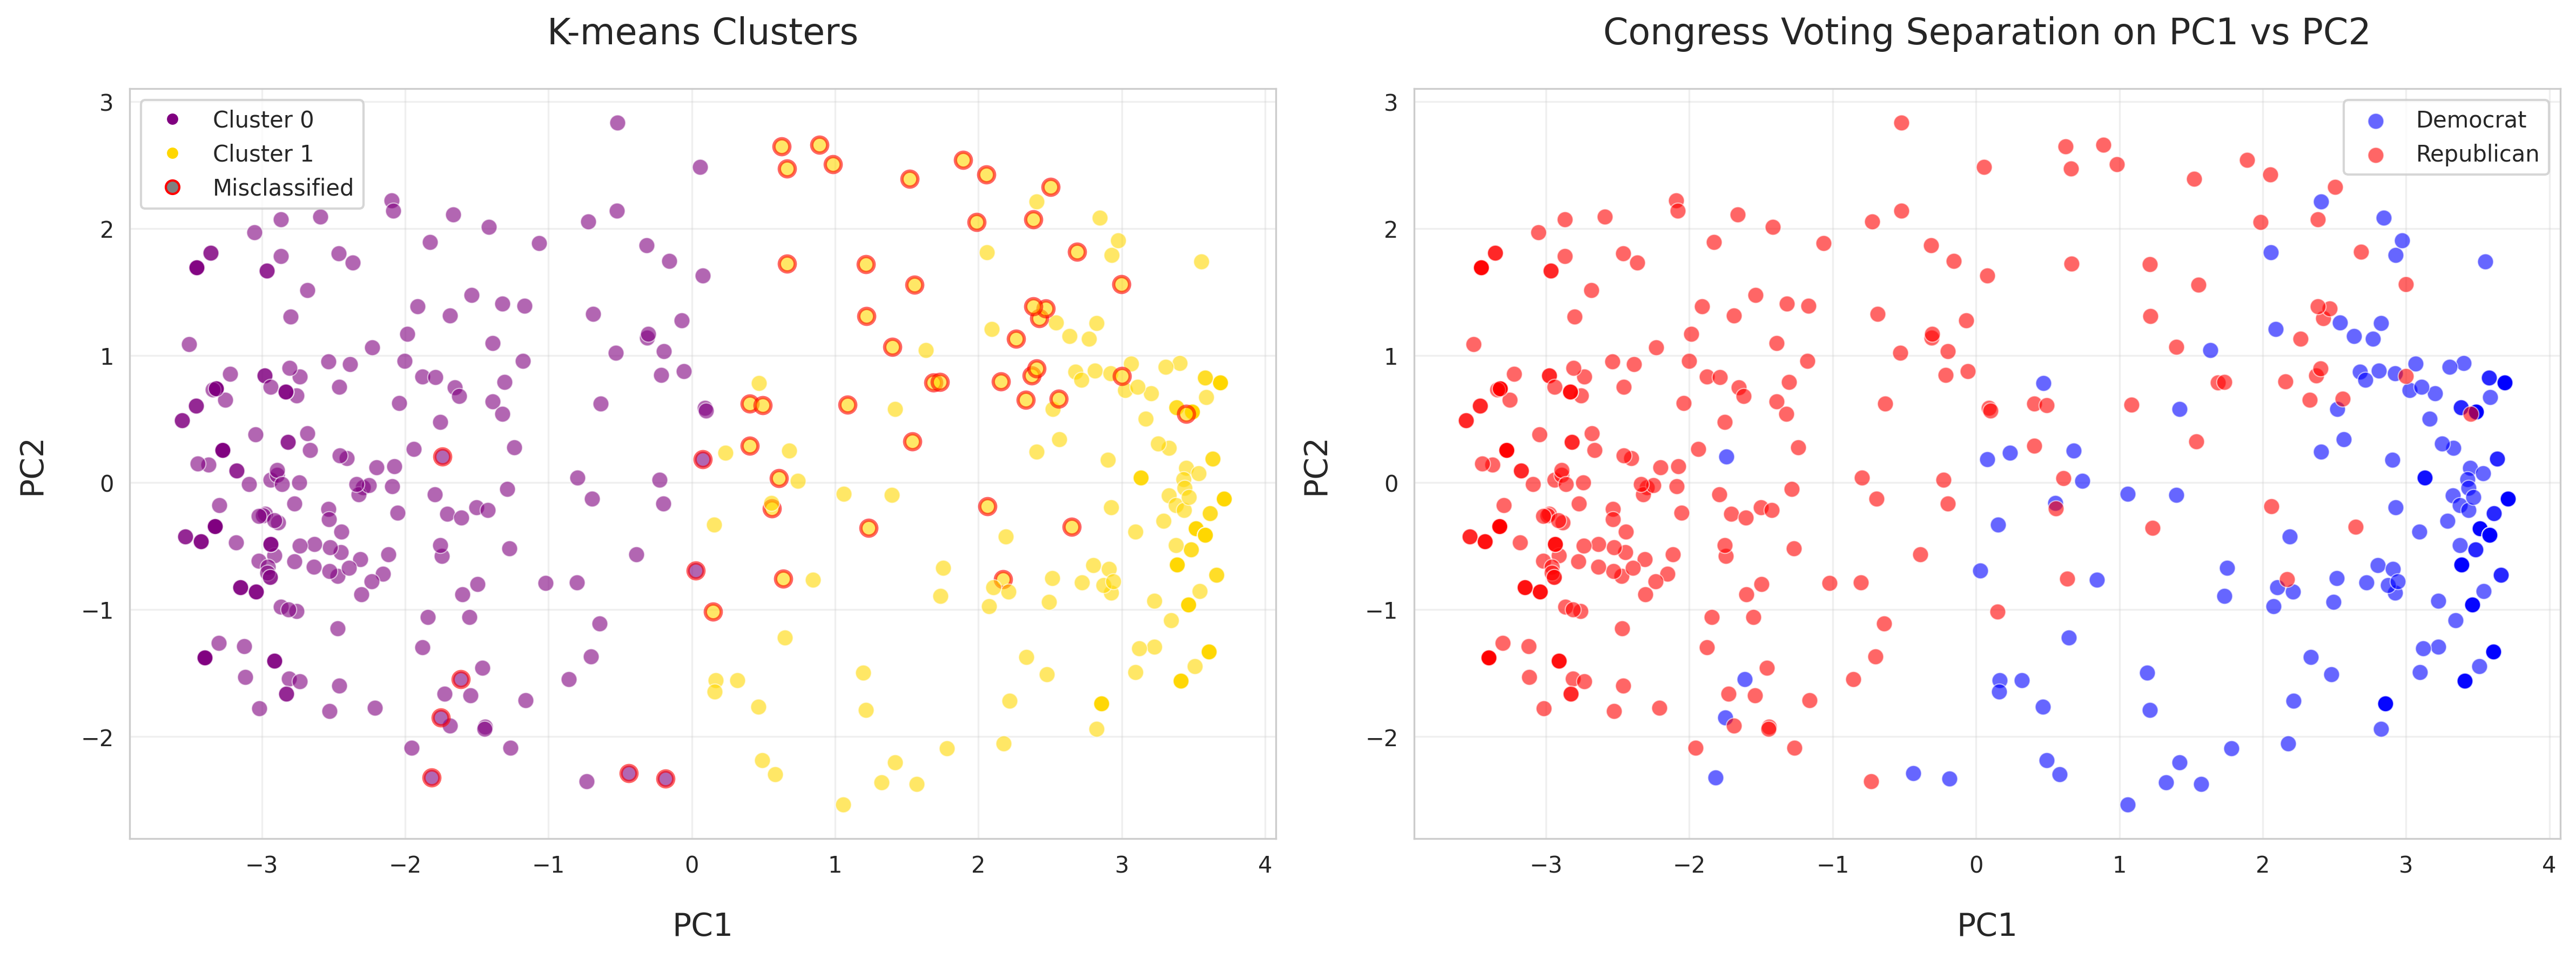
\includegraphics[width=0.95\textwidth]{figures/clusters_vs_parties.png}
  
  \textbf{Figure 8:} K-means clusters compared to party affiliations on PC1 vs PC2.
\end{center}

It is immediately apparent from the visual that the clusters are very well separated, very much along the PC1 origin boundary it appears. Regarding the party affiliations, kmeans is fairly weak to those members whose votings patterns stray from their parties, as it is the likely case that the centroids kept identifying these individuals as members of their cluster throughout the convergence due to their leaning behaviors. For that reason, I tried to capture the misclassification in the kmeans cluster overlay using red outlines, representing anyone regardless of party whose assigned cluster does not align with their political party. However, the voting patterns as they relate to party affiliation are still a rather good indicator, and so those whose voting behavior is as you would expected by party were largely assigned to the correct cluster, so I would still say the groups agree with their respective parties quite well.\\

To assess whether this clustering structure is statistically significant, I did exactly as the example in the instruction suggested and performed the permutation test using the objective function of the algorithm to measure the clustering quality. The observed result is 3778.34, and the implementation and visualization below show the score for 1000 permutations and their clusterings:

\begin{verbatim}
def permute_votes(votes: np.ndarray) -> np.ndarray:
    """
    Permutes votes randomly across issues for each congress member.
    
    :param votes: Original votes matrix
    :type votes: np.ndarray
    :returns: Permuted votes matrix
    :rtype: np.ndarray
    """
    permuted = votes.copy()
    for i in range(votes.shape[0]):
        permuted[i, :] = np.random.permutation(votes[i, :])
    
    return permuted


def permutation_test_clustering(votes: np.ndarray, n_permutations: int = 1000,
                                n_clusters: int = 2) -> tuple:
    """
    Performs permutation test for clustering significance.
    
    :param votes: Original votes matrix
    :type votes: np.ndarray
    :param n_permutations: Number of permutations
    :type n_permutations: int
    :param n_clusters: Number of clusters
    :type n_clusters: int
    :returns: Original inertia, null distribution, p-value
    :rtype: tuple
    """
    # Cluster original data
    _, _, original_inertia = cluster_kmeans(votes, n_clusters=n_clusters)
    
    # Generates null distribution
    null_inertias = np.zeros(n_permutations)
    for i in range(n_permutations):
        permuted_votes = permute_votes(votes)
        _, _, null_inertias[i] = cluster_kmeans(permuted_votes, 
                                               n_clusters=n_clusters,
                                               random_state=i)
    
    p_value = (np.sum(null_inertias <= original_inertia) + 1) / (n_permutations + 1)
    
    return original_inertia, null_inertias, p_value


def plot_permutation_results(original_inertia: float, null_inertias: np.ndarray,
                             p_value: float, output_filename: str):
    """
    Plots permutation test results.
    
    :param original_inertia: Inertia from original data
    :type original_inertia: float
    :param null_inertias: Null distribution of inertias
    :type null_inertias: np.ndarray
    :param p_value: Computed p-value
    :type p_value: float
    :param output_filename: Filename for output figure
    :type output_filename: str
    """
    sns.set_style("whitegrid")
    sns.set_palette("muted")
    plt.figure(figsize=(10, 6))
    
    plt.hist(null_inertias, bins=30, color='steelblue', 
             alpha=0.7, edgecolor='white')
    
    plt.text(0.95, 0.95, f'Observed: {original_inertia:.2f} (p = {p_value:.3f})',
            transform=plt.gca().transAxes, verticalalignment='top',
            horizontalalignment='right', fontsize=12,
            bbox=dict(boxstyle='round', facecolor='wheat', alpha=0.5))
    
    plt.xlabel('K-means Inertia', fontsize=14, labelpad=15)
    plt.ylabel('Frequency', fontsize=14, labelpad=15)
    plt.title('Distribution of K-Means Inertia for 1000 Permutations', fontsize=16, pad=20)
    plt.grid(True, alpha=0.3)
    
    plt.tight_layout()
    os.makedirs("../figures", exist_ok=True)
    plt.savefig(f"../figures/{output_filename}", bbox_inches='tight', dpi=300)
\end{verbatim}

\begin{center}
\textbf{Figure 9:} Vote permutation functions and visualization function for null distribution.
\end{center}

\begin{center}
  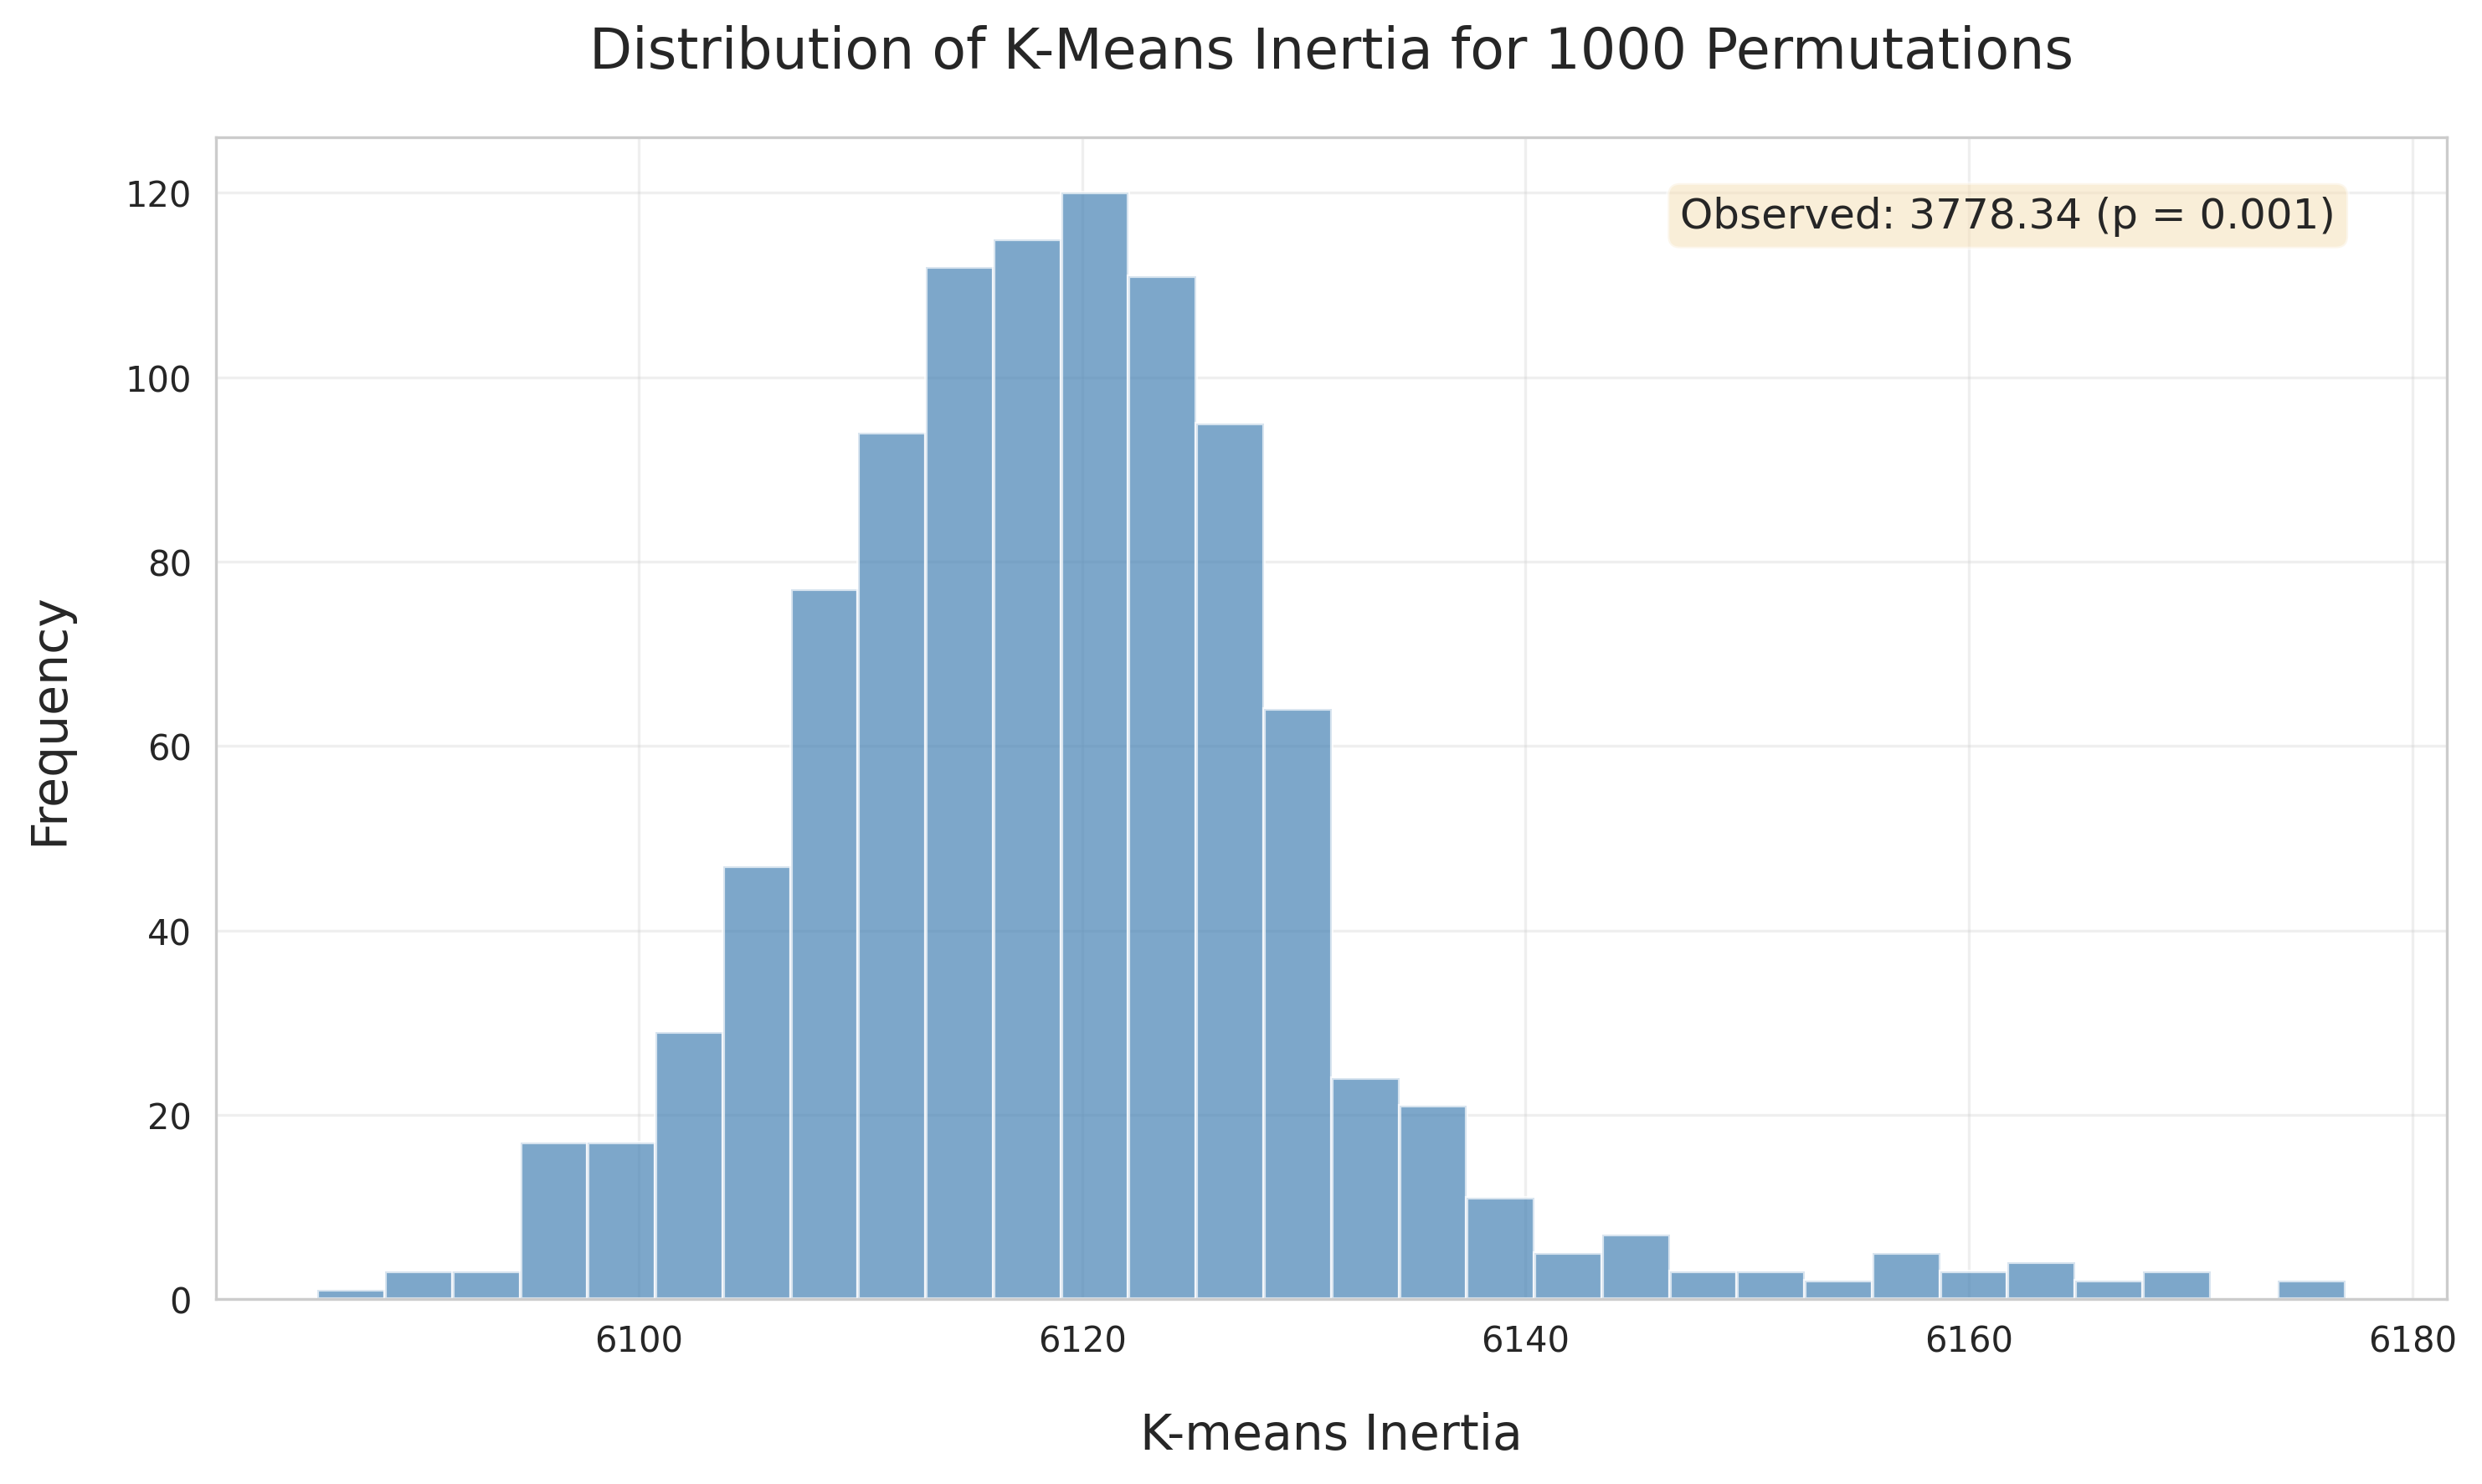
\includegraphics[width=0.95\textwidth]{figures/permutation_test_clustering.png}
  
  \textbf{Figure 10:} Null distribution of K-means inertia from permutation test.
\end{center}

The observed statistic is far lower than any value in the null distribution as expected from the discussion of the members whose voting patterns don't align with the affiliation, so for that reason I chose to exclude a visual marker of the observed statistic and left it as an annotation. Including it was ruining the scaling of the objective function axis and obfuscating the visual.\\

That being said, the observed statistic is far lower than the overwhelming majority of the distribution mass; where the average case measures at around 6120, the observed test statistic is only 3778.34. Along with its p-value of 0.001, the test result suggests that obtaining an observed clustering this strong is extremely unlikely under the null hypothesis, and we can reject. This indicates that the original data is significantly clustered.

\newpage
